%%
%% This is file `sample-acmsmall.tex',
%% generated with the docstrip utility.
%%
%% The original source files were:
%%
%% samples.dtx  (with options: `acmsmall')
%% 
%% IMPORTANT NOTICE:
%% 
%% For the copyright see the source file.
%% 
%% Any modified versions of this file must be renamed
%% with new filenames distinct from sample-acmsmall.tex.
%% 
%% For distribution of the original source see the terms
%% for copying and modification in the file samples.dtx.
%% 
%% This generated file may be distributed as long as the
%% original source files, as listed above, are part of the
%% same distribution. (The sources need not necessarily be
%% in the same archive or directory.)
%%
%% The first command in your LaTeX source must be the \documentclass command.
\documentclass[acmsmall]{acmart}
% NOTE that a single column version is required for submission and peer review. This can be done by changing the \doucmentclass[...]{acmart} in this template to 
% \documentclass[manuscript,screen]{acmart}

%to add images
\usepackage{graphicx}
\graphicspath{{Images/}}

%%
%% \BibTeX command to typeset BibTeX logo in the docs
\AtBeginDocument{%
  \providecommand\BibTeX{{%
    \normalfont B\kern-0.5em{\scshape i\kern-0.25em b}\kern-0.8em\TeX}}}

%% Rights management information.  This information is sent to you
%% when you complete the rights form.  These commands have SAMPLE
%% values in them; it is your responsibility as an author to replace
%% the commands and values with those provided to you when you
%% complete the rights form.
%%\setcopyright{acmcopyright}
%%\copyrightyear{2020}
%%\acmYear{2020}
%%\acmDOI{10.1145/1122445.1122456}


%%
%% These commands are for a JOURNAL article.
%%\acmJournal{JACM}
%%\acmVolume{37}
%%\acmNumber{4}
%%\acmArticle{111}
%%\acmMonth{8}

%%
%% Submission ID.
%% Use this when submitting an article to a sponsored event. You'll
%% receive a unique submission ID from the organizers
%% of the event, and this ID should be used as the parameter to this command.
%%\acmSubmissionID{123-A56-BU3}

%%
%% The majority of ACM publications use numbered citations and
%% references.  The command \citestyle{authoryear} switches to the
%% "author year" style.
%%
%% If you are preparing content for an event
%% sponsored by ACM SIGGRAPH, you must use the "author year" style of
%% citations and references.
%% Uncommenting
%% the next command will enable that style.
%%\citestyle{acmauthoryear}

%%
%% end of the preamble, start of the body of the document source.
\begin{document}

%%
%% The "title" command has an optional parameter,
%% allowing the author to define a "short title" to be used in page headers.

%WORKING TITLE FOR PAPER
\title[Privacy Preservation Analytics]{A Comprehensive Evaluation of Google's Differential-Privacy Tool on a Real-World Database}


%%
%% The "author" command and its associated commands are used to define
%% the authors and their affiliations.
%% Of note is the shared affiliation of the first two authors, and the
%% "authornote" and "authornotemark" commands
%% used to denote shared contribution to the research.
\author{Adithi Satish}
\affiliation{%
  \institution{PES University}
  \streetaddress{100 Feet Road, Banashankari Stage III, Dwaraka Nagar, Banashankari}
  \city{Bangalore}
  \state{Karnataka}
  \country{India}}
\email{adithisatish@pesu.pes.edu}

\author{Avnish Goel}
\affiliation{%
  \institution{PES University}
  \streetaddress{100 Feet Road, Banashankari Stage III, Dwaraka Nagar, Banashankari}
  \city{Bangalore}
  \state{Karnataka}
  \country{India}
}
\email{avnishgoel99@gmail.com}

\author{Manah Shetty}
\affiliation{%
 \institution{PES University}
  \streetaddress{100 Feet Road, Banashankari Stage III, Dwaraka Nagar, Banashankari}
  \city{Bangalore}
  \state{Karnataka}
  \country{India}
}
\email{manahshetty@gmail.com}

%%
%% By default, the full list of authors will be used in the page
%% headers. Often, this list is too long, and will overlap
%% other information printed in the page headers. This command allows
%% the author to define a more concise list
%% of authors' names for this purpose.
\renewcommand{\shortauthors}{Adithi Satish and Manah Shetty, et al.}

%%
%% The abstract is a short summary of the work to be presented in the
%% article.
\begin{abstract}
  With the world today advancing technology as fast as it is, data becomes the most priceless
resource, opening up a plethora of opportunities for companies and analysts to gain useful insights on the users and create better experiences and successful business models and strategies. However, improper disclosure of such data could be fatal while being a gross violation of the General Data Protection Regulation (GDPR) rules.
With this comes the ever rising need to create tools that facilitate the use of such sensitive data
without compromising users’ privacy. \newline
This project aims to appropriately test the differential privacy tool developed by Google and the
modifications made to it by Sriniketh M. Shenoy and Vikram G. on a real-time database and
comprehensively evaluates the claims made in enforcing differential privacy and improving the
performance overhead on the Google differential privacy tool, providing statistical and graphical
evidence for the same. Along with evaluation, it also seeks to determine the reasons for
malfunctioning and rectify it by making the appropriate modifications.
\end{abstract}

%%
%% The code below is generated by the tool at http://dl.acm.org/ccs.cfm.
%% Please copy and paste the code instead of the example below.
%%

\begin{CCSXML}
<ccs2012>
 <concept>
  <concept_id>10010520.10010553.10010562</concept_id>
  <concept_desc>Differential Privacy~Sensitivity</concept_desc>
  <concept_significance>500</concept_significance>
 </concept>
 %%<concept>
  %%<concept_id>10010520.10010575.10010755</concept_id>
  %%<concept_desc>Computer systems organization~Redundancy</concept_desc>
  %%<concept_significance>300</concept_significance>
 %%</concept>
 %%<concept>
  %%<concept_id>10003033.10003083.10003095</concept_id>
  %%<concept_desc>Networks~Network reliability</concept_desc>
  %%<concept_significance>100</concept_significance>
 %%</concept>
</ccs2012>
\end{CCSXML}

%%\ccsdesc[500]{Computer systems organization~Embedded systems}
%%\ccsdesc[300]{Computer systems organization~Redundancy}
%%\ccsdesc{Computer systems organization~Robotics}
%%\ccsdesc[100]{Networks~Network reliability}

%%
%% Keywords. The author(s) should pick words that accurately describe
%% the work being presented. Separate the keywords with commas.
\keywords{differential privacy, bounded user contribution, database, performance, accuracy}


%%
%% This command processes the author and affiliation and title
%% information and builds the first part of the formatted document.
\maketitle

\section{Introduction}\label{1}
In 2017, data surpassed oil to become the most valuable resource in the world. When Cambridge Analytica was exposed to have used user data from Facebook to intentionally try and manipulate (democratic) elections, the world saw just how catastrophic the consequences of breaches of users’ privacy and data leaks could be. Preserving users' privacy is the need of the hour and the right to protection of personal data was termed a fundamental right under the General Data Protection Regulation (GDPR) rules. 
\newline
At the same time, consumers also want high customization from their apps and services. On the other end, companies need to be able to grow their businesses by making insights about the data collected. This leads to a trade-off that needs to be achieved between the users, who want their personal data to be private, and the service providers, who need to make collective insights to evaluate their business models. Privacy-preserving analytics aims to provide a solution for the same by allowing companies to obtain collective results (for example, counts and averages), but denies the analyst access to any user’s individual data.

There are preexisting methods by which privacy can be preserved, including but not limited to, anonymization of data and k-anonymity. However, all these methods are highly susceptible to re-identification attacks and there is a significant risk of the users’ personal privacy being breached. An example of this would be the Netflix Prize dataset. Although anonymized, the dataset was subjected to re-identification via the IMDb dataset, which led to user identification details being revealed. This stressed on the need for a new method of privacy preservation; one that was not susceptible to privacy breaches; the result of which introduced the concept of differential privacy. 

Differential privacy, in layman’s terms, states that {\itshape the presence or absence of any single individual’s data should not have a measurable effect on the results of a query}. This provides precise answers to queries about the population of the dataset without revealing much about any individual. It is widely regarded as the best way to preserve privacy, making use of several different mechanisms to do so. Fundamentally, differential privacy adds a certain amount of noise to a query’s results before displaying it to the user, thus protecting privacy. This noise can be drawn from various distributions (Laplace being the most common) and is scaled to the sensitivity of each query using the privacy budget. 

The privacy budget (epsilon) is the factor by which differential privacy is preserved. It has been found that the lower its value, the more private the results are. However, it has an inverse effect with the accuracy of the results. The privacy budget is extremely important in calculating the amount of noise to be added to the result, which is usually scaled by the aggregation’s sensitivity.

Some existing mechanisms which enforce differential privacy are PINQ (Private Integrated Queries), wPINQ, Sample and Aggregate, Restricted Sensitivity and Elastic Sensitivity. Tools like FLEX and CHORUS (in deployment at Uber) make use of these mechanisms to preserve privacy. Google’s differential privacy tools draws inspiration from the same mechanisms, but uses a different set of algorithms to enforce differential privacy. 

However, these differential privacy mechanisms have been found to incur a lot of performance overhead, thereby reducing the efficiency of the tool. Significant overhead is the result of the Sample and Aggregate mechanism, one which enforces differential privacy on aggregate functions like SUM and AVG. Google’s tool, which involves a mechanism to clamp the data points within a certain range, uses histograms to do so, resulting in almost 500x performance overhead. The changes proposed to Google’s tool however, claim to significantly reduce this overhead. The tool also fails to support queries that depend on more than one of these mechanisms, like the ones that involve both counts and aggregations. Elastic sensitivity does not support non equijoins and can be applied only when the join keys are drawn directly from the table.
\newline
Hence, a comprehensive evaluation of the tool on a real world database is absolutely necessary before deploying the same in the industry. The tool has to be tested on every aspect, from the algorithms used to the performance and right down to the documentation and installation process. This project aims to evaluate the tool on a database similar to the ones used by service providers in the industry, by testing not only the mechanisms used, but all other aspects, choosing relevant criteria for the same.


\section{Literature Survey}\label{2}
\subsection{Towards Practical Privacy-Preserving Data Analytics}\label{2.1}
This thesis\cite{Johnson2018TowardsPDP} provides a complete explanation of all the fundamental concepts related to differential privacy. It also explains the working of the existing mechanisms like wPINQ and Sample and Aggregate. Additionally, it introduces two new concepts: Elastic Sensitivity, and CHORUS: a differentially private engine that uses Query Rewriting. 

Sensitivity is defined as the maximum difference in the results of a query on two databases. Sensitivity applied on any two neighbouring databases is termed ‘global’, and is termed ‘local’ when applied on the true database with any neighbouring database.
Local sensitivity is the preferred measure to scale down noise since it reflects the true database. However, it is computationally costly on queries with joins. Hence, an upper bound on local sensitivity called ‘elastic sensitivity’ is used.
Laplace noise scaled to elastic sensitivity is added to the results of a query in order to get differentially-private results. The thesis introduces FLEX, a mechanism that uses elastic sensitivity. 

CHORUS is a privacy preservation tool that achieves differential privacy via query rewriting. It embeds the intrinsically private query with a differential privacy mechanism before execution, thus successfully side-stepping the hassle of post processing. It involves two main steps : (1) Mechanism Selection and (2) Query Rewriting as shown below :

\begin{figure}[htp]
    \centering
    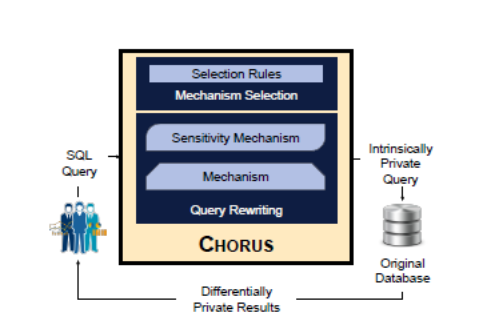
\includegraphics[width=5cm]{Fig 2.1.1.png}
    \caption{Working of CHORUS}
    \label{fig:2.1.1}
\end{figure}

The query is analysed and a parser helps select the mechanism to be deployed accordingly. CHORUS integrates all the commonly used mechanisms and is adaptable to any SQL engine. This architecture works very well, covering most real world queries and is currently in place at Uber. However, the performance overhead on queries involving aggregations can be improved upon. The current overhead on such queries is extremely high due to the computational costs of splitting the database into chunks and running queries on each chunk followed by the aggregation.

\subsection{Differentially Private SQL with Bounded User Contribution}\label{2.2}
This paper\cite{wilson2019differentially} provides an in-depth explanation of the concepts used by Google's differential privacy tool. It is founded on the principle that the presence or absence of a single individual does not affect the aggregate. However, this holds true only when the contribution of every individual in the database is uniform and fails when a single individual can be associated with more than one database record. This is not true of most real-world databases. The paper proposes an SQL Engine that overcomes this pitfall by binding the contribution of every user to a certain value and scaling sensitivities accordingly and thereby enforcing differential privacy at the user level.

In order to overcome the unbounded sensitivity that arises due to multiple contributions by a user to a partition, the contributions by every user is bounded, and noise levels are accordingly adapted.
However, this does not protect from a privacy breach of those users with single or low contributions. In such a case, privacy can still be breached in comparison with another database that does not have this particular user. Hence, all keys associated with a noisy count lower than a certain threshold are also dropped.  In addition to the above, a single user could also contribute to multiple partitions, changing the sensitivity of a query from one to the number of partitions. The paper introduces a mechanism to bound this as well.

A query rewriter is used to validate anonymization semantics and enforce them. The query rewriter first checks if each row is owned by a single user and then evaluates the subquery. It then performs a partial aggregation using GROUP BY on the resultant relation based on the user identifier chosen (special column added). A fixed number of rows are then sampled from each user to limit the user contribution across partitions. Finally, a cross-user DP aggregation, across all the users, is computed from the resultant relation while now limiting user contribution within a partition.

The engine further uses a function - Approx Bounds, to calculate the optimum lower and upper bounds with minimum cost to accuracy of the result. The data is thus clipped according to the bounds thereby preserving differential privacy by limiting a single user’s contribution to the aggregate while also possibly having a positive effect on the data model by removing outliers. The presented system enforces user-level differential privacy. It is able to implement most data analysis tasks based on aggregations. The paper also presents a stochastic tester whose results further strengthen the made claims on preservation of privacy. 

\subsection{Privacy-Preserving Analytics}\label{2.3}
This paper\cite{srinivikram2020ppa}, by Sriniketh Shenoy and Vikram G, analyses Google's differntial-privacy tool (Section 2.2) and introduces modifications to the same in order to combat the performance overhead incurred by the tool. 

The design approach followed is a sequential one, with emphasis on accurate change measurement and eliminating existing problems. At an abstract high level, the tool consists of two modules, the Pre-Processor and the Privacy Preserving Engine. The former, which is a wrapper around Google's tool, accepts the SQL query and parses the same according to the semantic specifications of the engine. It also converts WHERE clauses to respective INNER JOINs, which is known to have performance improvements. The latter enforces differential privacy either using Bounded or Unbounded mechanisms, adding Laplace noise to obtain differentially private results. 

\begin{figure}[htp]
    \centering
    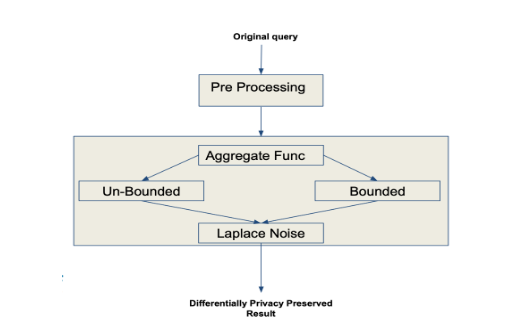
\includegraphics[width=5cm]{Fig 2.3.1.png}
    \caption{Working of Tool and Wrapper}
    \label{fig:2.3.1}
\end{figure}

Functionalities of the tool that are analysed include, stress testing, user friendliness, functional testing, error handling and bounded value testing. The paper makes claims about the time taken for processing of normal, bounded and unbounded queries, accuracy of results obtained and preservation of users' privacy. 

The paper includes sections about the results of the minimal testing carried out, claiming that the wrapper significantly improves the performance overhead incurred by the tool and also sets the Margin of Error as 20\%. From here on, Google's differential privacy tool will be referred to as plainly, the tool, whereas the modifications made will be referred to as the wrapper. 

The paper also highlights where the wrapper/tool fails, and it is hence, imperative to test both on a real-world database to see if the claims made by the authors do indeed hold up. 

\section{Criteria for Evaluation}\label{3}
The criteria for evaluation is subdivided into six broad categories which deals with every part of the tool, from its performance and accuracy to the installation process and documentation. The categories are as follows:
\begin{itemize}
    \item 
    \textit{Need: } Analysis of the problem statement is the first step in the evaluation of any tool. It helps us understand the issue at hand, and why there is a need for this particular software/tool in the industry.
    \item
    \textit{Methodology: } This category aims to analyse the fundamental algorithms behind the tool, and dwells upon the theoretical knowledge behind each algorithm. It also seeks to juxtapose the Google algorithms with the changes made by the authors of the wrapper.
    \item
    \textit{Adaptability: } Evaluation of the tool’s build process is handled under this category, in order to check what the tool’s dependencies (software and hardware) are, and if true,  highlight the areas of failure to build.
    \item
    \textit{Functioning: } One of the main categories, it involves evaluating the tool on the above-mentioned database to check its functioning and if the tool malfunctions under any situation. If the tool indeed fails for some test cases, it aims to find the reason for the same.
    \item
    \textit{Performance and Accuracy: } The crux of the evaluation lies with the tool’s performance and accuracy. The main goal is to inspect if the claims made by the authors of both the tool and the wrapper do indeed hold up when tested on a real-world database, supporting the same with graphical and statistical evidence.
    \item
    \textit{Usability: } This category deals with the general evaluation of the tool, with regard to how user-friendly the interface is, as well as the tool’s documentation and provisions to report bugs and grievances faced, and the ease of making modifications.
\end{itemize}

The following sections elaborates on each of these categories, along with suggesting changes and modifications that can be implemented as future scope. 

\section{Evaluation}\label{4}
The tool is evaluated based on all the criteria listed above, and tested to check if both the tool and the wrapper satisfy the claims of the authors. The evaluation process is a comprehensive one, from the tool's performance right down to its documentation and installations. The following subsections illustrates the same and provides results of the tests carried out.

\subsection{About the Tool}\label{4.1}
The Google Differential Privacy Tool contains a set of libraries of \begin{math}\epsilon\end{math} - and \begin{math}(\epsilon, \delta) \end{math}- differentially private algorithms which can be used to perform aggregate queries on numeric data sets with private or sensitive information.The tool algorithms, modifications and drawbacks have been explained in detail below.
\newline
\newline
\textbf{Tool Algorithms and Mechanisms}:
\newline
\newline
\textit{What are the algorithms used by the tool?}

The tool makes use of query rewriting to enforce differential privacy using algorithms that depend on bounded user contribution. Bounded user contribution limits the contribution of each user to the output. It does so by setting appropriate upper and lower bounds and clamping all the values in the dataset between these two bounds. Once these new values are calculated, the aggregation is performed on them and finally, Laplace noise scaled to the sensitivities of these new values is added to produce the differentially-private result.

The tool requires queries to be passed in accordance with the new semantics that the algorithms define. For example, a query that makes use of the SUM aggregation would have to be passed using the ANON\textunderscore SUM function.
\newline
\newline
\textit{An example of working of the mechanisms}

Consider a query passed using which the analyst wants to determine the SUM of a particular attribute (att) of a relation (R). To obtain non-differentially private results, the analyst would simply pass the following query to his SQL engine:
\begin{center}
    SELECT SUM(att) FROM R
\end{center}
The differentially private version of this query would resemble something similar to:
\begin{center}
    SELECT ANON\textunderscore SUM(att) FROM R
\end{center}
The working of the algorithm is as follows:
\begin{itemize}
    \item Lower and upper bounds are assigned. The user can pass these bounds as parameters in the ANON\textunderscore SUM aggregation and if not, the bounds are calculated using histogram bin enumeration by the tool itself, using a part of the privacy budget to do so.
    \item The values are clamped between these upper and lower bounds using the Winsorized mean technique as: x’ = MAX(L, MIN(U, x)).
    \item The aggregation function (non differentially private), in this case SUM is applied on these newly obtained values.
    \item The sensitivity(S) of the differentially private algorithm is determined by the bounds. For ANON\textunderscore SUM, the sensitivity has been determined to be max(|L|,|U|).
    \item To the obtained result of the SUM aggregation, Laplace noise scaled to the sensitivity is added as Lap (S/e). This is the final differentially private result that is returned to the analyst.
\end{itemize}
Similar procedures are followed for all other aggregation functions too.
\newline
\newline
\textit{How are the bounds approximated?}

If the user does not provide the lower and upper bounds, they are calculated using the ApproxBounds algorithms. Contiguous histogram bins are created with appropriate bin labels into which the input values are partitioned. A threshold count value is obtained using a mathematical expression [\ref{Appendix. C}].
Max and min are approximated using only those bins whose noisy count exceeds the threshold. The upper bound maps to the bin containing the largest values with noisy count greater than threshold, and similarly, the lower bound maps to the bin containing the smallest values. On evaluation, it was found by the authors that calculations of the ApproxBounds were responsible for the significant performance overhead of the tool.
\newline
\newline
\textit{Are the algorithms comprehensive and well documented?}

With regard to the complexity of the algorithms, the result performance, as mentioned in the documentation, is O(n) for all the Bounded mechanisms. The tool contains documentation for each of the Bounded algorithms used which is brief and provides enough information about the working of the same. At the high level documentation, links to articles and blog posts about differentially privacy are provided. The paper that resulted from this research, “Differentially Private SQL with Bounded User Contribution” explains in detail the need for these algorithms, an in-depth working of the same, and also provides a comparison between the tool and other differential privacy mechanisms like wPINQ.
\newline
\newline
\newline
\textit{What are the tool’s drawbacks?}

Google’s differential privacy tool makes use of algorithms defined in a way that leaves it incapable of assessing normal SQL queries. Instead, the ANON version of the same is required to satisfy the tool semantics. This doesn’t leave a lot of room for adaptability. The tool is also dependent on PostgreSQL 11, and does not work on any other RDBMS engine, nor does it support a different version of PostgreSQL. 
Coming to its performance, the tool incurs very high performance overhead, with the time taken to process a differentially private query being almost 500x the time taken to process a normal query. On further analysis, it was found by the authors that the ApproxBounds algorithm was the reason for the same, as histogram bin enumeration is taxing and can result in a lot of overhead.
\newline
\newline
\textit{What are the changes made?}

As mentioned above, the tool has certain limitations when it comes to the type of queries that can be passed and the performance overhead incurred. The changes proposed and later, implemented by the authors were
\begin{itemize}
    \item A parser written in Python, which accepts normal SQL queries from the user/analyst and converts them into the differentially private queries required by the tool.
    \begin{itemize}
        \item In order to reduce performance overhead, any SQL statements involving a WHERE clause with multiple tables is changed to an INNER JOIN with the corresponding condition.
        \item Similarly, any query containing the NOT IN clause is converted to a specific WHERE logic.
    \end{itemize}
    \item The major cause of performance overhead was found to be the ApproxBounds algorithm used to automatically calculate the lower and upper bounds when these values are not passed as parameters to the ANON aggregation. To improve this, an Unbounded/Fastbounded mechanism is proposed, which approximates the lower and upper bounds using a MinMax function, which claims to result in significant improvement of overhead.
\end{itemize}
The changes made do not modify any of the fundamental differential privacy algorithms that the tool uses; it is instead a wrapper that allows the analyst to pass normal SQL queries to the tool and obtain a differentially private result.

The new algorithm defined in the wrapper to calculate lower and upper bounds uses a MinMax mechanism, where the lower bound is set to the minimum value and the upper bound is set to the maximum value found in the dataset. This can, in some cases compromise on the differential privacy that the tool promises. This is due to the fact that the MinMax algorithm considers the outliers in the dataset instead of clamping them between a certain range. Outliers in any dataset are found to heavily influence the result of aggregations and hence do not conform to the definition of differential privacy, which states that any one value should not have a measurable effect on the result. Hence, the MinMax mechanism deals with the trade-off between performance improvement and preservation of privacy by undermining the latter in order to improve the former.

A modification that we suggest as an alternative for both MinMax and Histogram Bin Enumeration is the Widened Winsorized Mean method, where the bounds of the interquartile range can be taken as the respective lower and upper bounds. This will definitely negate the effect of outliers and may also provide significant improvement on the performance overhead from the ApproxBounds method. Although it may not provide as much improvement as the MinMax method and the accuracy of the result obtained may have a larger margin of error, it does not compromise the users’ privacy.
\newline
\newline
\newline
\textbf{Tool Installation and Build Procedure}

Google’s privacy preservation tool is available open source on GitHub, however the tool must be built prior to execution of queries. Due to the absence of a single .exe file that would otherwise take care of the installation, the entire tool has to be built step by step. The procedure to build is not extremely straightforward due to the tool’s many dependencies. The software dependencies include Bazel v.3, PostgreSQL v.11, Bison Flex in addition to the requirement of Linux for installation. It is imperative to note that if any of these requirements are not satisfied, the tool will fail to build. Perhaps the most glaring disadvantage is that the tool requires extremely fast and stable internet speed, and will fail to build with the slightest fluctuations of the same, usually resulting in BoringSSL errors.
\newline
\newline
\textit{Common Issues}
\begin{itemize}
    \item Fluctuating internet issues was the main problem we faced during installation, with random BoringSSL errors popping up as a result of failure. However, the internet bandwidth in companies is usually very stable and hence this issue becomes redundant.
    \item Installation procedure is not very straightforward; the process involves a lot of steps that require superuser/administrator privileges and the installation process comes to a standstill without these requirements being satisfied.
    \item The extension has to be created for every database that exists, and will not work if created only for the user that the databases fall under.
    \item Even after “successful” build messages, there may be some errors while trying to execute the parser and the extension. For a user who has only the high-end knowledge of the tool’s algorithms, pinpointing the cause of these errors can be very taxing, with debugging even more of a daunting task. While installing the tool and doing dry runs of the same, we came across a couple of these errors, which we had a hard time resolving.
    \item Some errors(eg: PostgreSQL errors)  caused by intermediate steps can’t be resolved without redoing the entire build process from scratch, which turns out to be a hassle.
\end{itemize}

Installation of the tool was found to be an exhaustive process and had to be redone multiple times before successfully installing it on the system. An .exe file would make the whole process much simpler and not dishearten users who are unsuccessful in building the tool. Even a Docker image would be a helpful alternative to the build process. It would package up the code and all its dependencies so that the application runs quickly and reliably on any computing environment. This would make the entire procedure single-step while being light and stand alone.
\newline
\newline
\textbf{Enhancements}

Upon evaluation of the algorithms and functioning of the wrapper[\ref{4.3}], a few errors came to light and modifications were made to the wrapper by the evaluators to deal with a few of these[\cite{adithi2020ppa}].

One of the glaring errors posed by the wrapper, as will be elaborated in section \ref{4.3} is with respect to dealing with queries that include string matching. Upon examination of the wrapper, it was found that the entire query is converted to the lower case raising problems with queries that match strings with upper case characters. The wrapper function to set bounds, requires a query rewrite by performing a split on the query based on the type, because of which the query as a whole, was set into the same case by the authors. This has been dealt with by retaining the query as it is and performing a check on the case of the ‘type of query’, without modification to the same, only in the concerned section of the wrapper function to set bounds. This error has thus been successfully debugged and the wrapper and tool now function smoothly for such queries.

Another blatant error that surfaced upon examination of the algorithms in place in the wrapper was the threat to the privacy of users. The wrapper includes a ‘FastBound’ mechanism to approximate the bounds passed to the ANON aggregate function to significantly reduce the performance overhead. While this is successfully achieved, a significant compromise on the users’ privacy is incurred while doing so. This is because the FastBound function uses a MinMax mechanism to set the bounds. It queries the database for the minimum and maximum value of the attribute of interest and sets this as the lower and upper bounds to the anon function. An example of this conversion is as follows:
\newline
Consider a simple query -
\begin{center}
    SELECT AVG(price) FROM completeride;
\end{center}
The FastBound function modifies the query and sets the lower and upper bound, respectively,  as follows :
\begin{center}
    SELECT MIN(price) FROM completeride;
    SELECT MAX(price) FROM completeride;
\end{center}
This approach could possibly lead to a gross violation of the concept of differential privacy due to its inclusion of all the records in the database, specifically the outliers. Outliers represent the extreme values in a dataset and have a significant impact on the results of an aggregate query. Inclusion of outliers hence violates the concept of differential privacy which states that the presence or absence of an individual record should not have a measurable effect on the result of an aggregate query. Therefore, while the FastBound mechanism significantly improves the performance overhead, it does so while undermining user privacy since the noise added is not appropriately scaled to protect privacy.
 
The evaluators have come up with a Widened Winsorized Mean mechanism to deal with the same. The wrapper has been modified to set the lower and upper bounds as the 15th and 85th percentiles of the attribute of interest. The mechanism converts the aforementioned query to set bounds as follows: 
\begin{center}
    SELECT percentile\textunderscore cont(0.15) within group(order by price) FROM completeride;
\end{center}
\begin{center}
    SELECT percentile\textunderscore cont(0.15) within group(order by price) FROM completeride;
\end{center}
This mechanism keeps with the concept of differential privacy since it clamps the outliers to lie within a certain range nullifying the impact of any single record on the aggregate. The range chosen is an extension of the optimum inter-quartile range widely used in data science and thus represents the model of the dataset justly, despite the clamping. While this mechanism has a higher performance overhead when compared with the FastBound mechanism, it triumphs in its preservation of user privacy as well, while achieving a performance overhead significantly better than the Bounded mechanism used by the tool. The evaluation of the same can be found in section \ref{4.4}.

\subsection{About the Database}\label{4.2}
The database used in this evaluation was a sample “uber” database, intended to be a representation of the multinational service-provider’s database. It includes relations like “driver”, “passenger”, “car” with relevant details about the same. Other relations include “completeride” which holds records of all the rides taken, “curride” which has information about a customer’s current ride, with attributes like pickup point, destination, pricing and surge.

With regard to the size of the database, all the eight relations, except for the “requests” relations have 50,000 to 100,000 records, which is small as compared to big companies, but is comparable with databases of startups. Taking all these factors into account, it can be concluded that the sample test database is indeed a satisfactory representative of a real-world database used by all major service providers.

However, all these relations contain extremely sensitive information about not only the passengers and their rides, but also the drivers. The relation “card\textunderscore” has credit card details of the passengers, which, if compromised can be catastrophic.

The “requests” relation is the smallest table in the database, with only 100 records. The tool, however, can handle queries that process a minimum of 200 records or higher, and fails to work when that requirement isn’t met. Hence, queries that are written to perform analysis on the “requests” table will fail to provide differentially private results. However, the attributes mentioned in the schema of the relation are also included in the schema of other relations in the database, so analysis can be performed on them in order to gain relevant insights from the data collected.
\newline
\newline
\textit{Industry Relevant Queries}

Upon evaluation of the database and its schema to confirm if it is a satisfactory representation of databases used in the industry, the next step involved querying the database on various aspects as analysed from the schema. These queries resembled ones being used by analysts in the industry, to make relevant insights about the data collected. The UC Berkeley thesis was referred to while writing the most optimal queries, and their performance. The authors of this thesis performed analysis on a dataset containing 8 million queries that are most commonly used by data analysts at Uber. 

With regard to the types of queries, the literature survey showed that the most frequent relational operators used in queries (excluding SELECT) was the JOIN operator, followed by the UNION and EXCEPT operators.

\begin{figure}[htp]
    \centering
    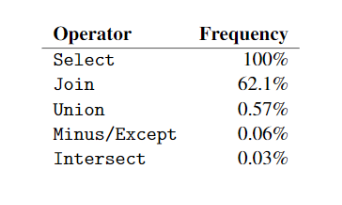
\includegraphics[width=5cm]{Fig 4.2.1.png}
    \caption{Frequency of Relational Operators}
    \label{fig:4.2.1}
\end{figure}

A significant number of queries also made use of multiple joins, with the number of joins in a query going up to almost 100. However, most queries made use of 0 to 25 join clauses. Equijoins accounted for more than 75\% of the joins performed, with the inner join being the most frequently used join operation. Self joins accounted for just 28\% of all join queries.

With respect to the aggregations, analysis performed by the authors of the thesis showed that only 34\% of all queries gave statistical results, i.e, made use of the aggregation functions. The rest of the queries resulted in raw data in at least one column. The latter, cannot be used in evaluation of the tool as differential privacy does not allow the analyst to access any raw data.

\begin{figure}[htp]
    \centering
    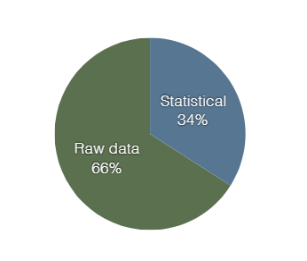
\includegraphics[width=5cm]{Fig 4.2.2.png}
    \caption{Types of results returned by typical queries}
    \label{fig:4.2.2}
\end{figure}

SQL provides analysts with a host of aggregation functions that are used to perform statistical analysis on the population of a dataset. Some of the most commonly used ones include COUNT, SUM, AVG, MAX and MIN. The frequency of the respective aggregations is as shown below, with more than half of the aggregation queries making use of COUNT; SUM coming in second.

\begin{figure}[htp]
    \centering
    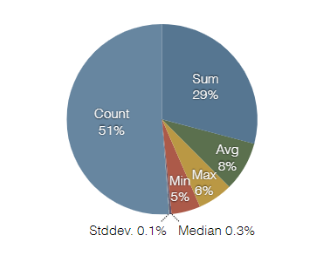
\includegraphics[width=5cm]{Fig 4.2.3.png}
    \caption{Frequency of Aggregates}
    \label{fig:4.2.3}
\end{figure}

Most queries are not very complex, having 4-10 clauses. However, analysis found that there are a small number of queries with over 100 clauses. The results of queries also follow a similar pattern, with most having less than 100 rows and columns. Queries returning just 1 value were found to be the most common.

There is a need to test the tool on non-differentially private queries to see where it fails and also note the performance of the same. In order to do this, around 50 queries were considered, satisfying the inferences drawn from the analysis performed in the thesis. Each of these queries have significant relevance with the database and have been written in such a way that they can be used in the industry as well. Each  query was run 10 times and the average of all the execution times of each run was considered to be the performance of said query. 

The tool was tested for performance and accuracy over the execution of simple queries with and without aggregation functions like SUM, AVG, MIN, MAX as well as complex queries with nesting upto 5, with and without aggregation functions, GROUP BY and JOIN clauses.

The queries have been designed keeping in mind their relevance in the industry. They reflect and provide insights on certain trends to help analysts market better and model the business to target more customers and increase outreach. The queries cover the most popular pickup spots, peak times, highest paying rides, revenue from a certain locality etc. They also cover the relationship between comfort of travel and revenue, number of bookings, working hours, ratings, the relationship between working hours and income, surges in price and number of bookings. The queries could help keep track of all the vehicle models and updations required, provide foresight on the kind of vehicles to invest on, the localities to frequent to adjust for bottlenecks and other common issues, formulate strategies to set fares dynamically, provide offers as well as predict supply and demand in order to make the perfect business model.

The same queries were then tested with respect to preservation of privacy, to see if the claims made by the developers and the authors who made modifications to the same, held up. The differentially-private queries were compared with the non-private ones, with reference to the accuracy of the results obtained, and the performance overhead incurred by the tool and the wrapper.


\subsection{Functioning of the Tool}\label{4.3}
Various queries were run on the tool to evaluate its functioning. These queries were designed from an industrial and business perspective, and range from simple queries with just one aggregate function to queries with multiple joins, aggregations and almost 5 nested clauses. The wrapper was modified so as to return the result and execution time of all the algorithms the tool supports: i.e normal (non-differentially private), Bounded, FastBounded and Widened Winsorized mechanisms.

The simple queries ran without any hassle on the tool, and provided the necessary output. For queries that would ideally compromise on user’s privacy, the tool does not return any result, rather, an NaN value is obtained, satisfying the claims of differential privacy made by the tool and wrapper.
Shown below is an example of the same:

\begin{figure}[htp]
    \centering
    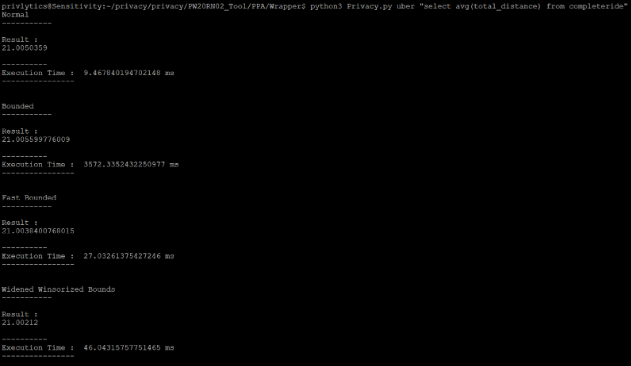
\includegraphics[width=7cm]{Fig 4.3.1.png}
    \caption{Example of the tool processing a simple query}
    \label{fig:4.3.1}
\end{figure}

The above query, \texttt{SELECT AVG(total\textunderscore distance) FROM completeride} is representative of commonly used queries in the industry to find the mean of a dataset. With respect to the test database, this query aims to find the mean of the total\textunderscore distance covered in each ride, from the pickup point to the destination. The above snapshot is proof of the tool’s functioning and the variance in the result provides ample proof of the user’s privacy being preserved. Analysis of the accuracy and performance overhead of the algorithms is done, in detail in the following section. 
The wrapper was not tested on simple aggregate queries alone, rather on a host of different queries as mentioned above. An example of a quintessential nested query run on the tool is \texttt{SELECT COUNT(driver\textunderscore id) FROM driver WHERE (lisence\textunderscore plate IN (SELECT lisence\textunderscore plate FROM car WHERE(model\textunderscore id IN (SELECT model\textunderscore id FROM size\textunderscore x WHERE model\textunderscore name = 'Mercedes E-class')))) AND avg\textunderscore ratings = 5;}, which gives the analyst the count of all the drivers who drive a Mercedes E-Class and have an average rating of 5.

\begin{figure}[htp]
    \centering
    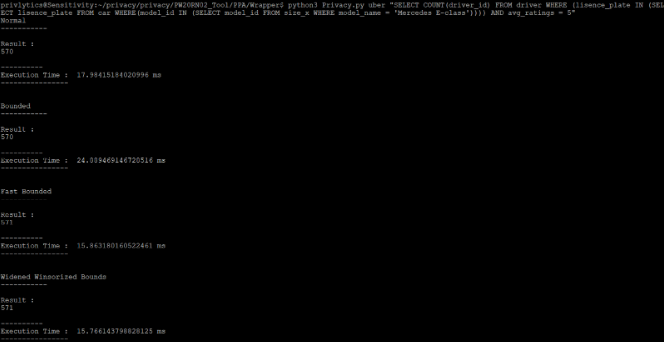
\includegraphics[width=7cm]{Fig 4.3.2.png}
    \caption{Output of tool for the nested query}
    \label{fig:4.3.2}
\end{figure}

The tool was evaluated on queries with JOIN clauses as well. An example of the same is a query written to count the number of rides priced greater than \$50, which were serviced by a driver with a rating of 4 or higher. This involves the join of relations ‘driver’ and ‘completeride’ as follows: \texttt{SELECT COUNT(*) FROM driver JOIN (SELECT driver\textunderscore id FROM completeride WHERE price > 50) AS n1 ON driver.driver\textunderscore id = n1.driver\textunderscore id AND avg\textunderscore ratings > 4;}. It’s interesting to note that the query not only has a join clause but also involves a nested clause. The output of passing the query to the wrapper is displayed in the snapshot provided below.
%Insert Fig 4.3.3
\begin{figure}[htp]
    \centering
    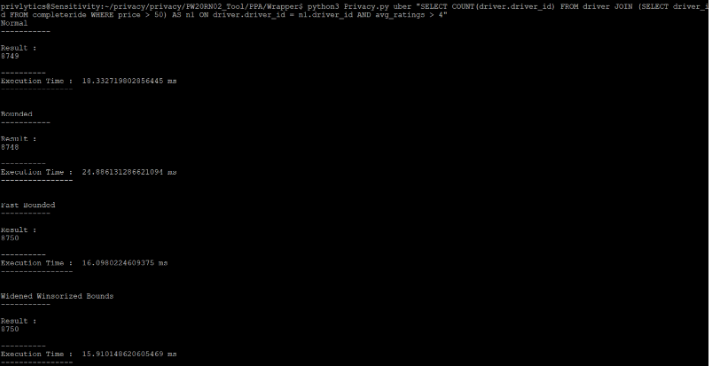
\includegraphics[width=7cm]{Fig 4.3.3.png}
    \caption{Output of tool for query with joins}
    \label{fig:4.3.3}
\end{figure}

However, the wrapper fails to work for certain queries, which can be problematic as an analyst without sufficient information about the wrapper’s working would be incapable of debugging these errors. One glaring error posed by the wrapper is the conversion of the entire query to lowercase without consideration of any string matching that may have to be performed. For example, the query, \texttt{SELECT COUNT(lisence\textunderscore plate) FROM car WHERE lisence\textunderscore plate LIKE 'MDO\%'}, is converted entirely to lowercase by the wrapper, resulting in \texttt{SELECT ANON\textunderscore COUNT(lisence\textunderscore plate) from car WHERE lisence\textunderscore plate LIKE 'mdo\%'}. The strings to be matched are different and hence, the results returned are wrong.
%Insert Fig 4.3.4
\begin{figure}[htp]
    \centering
    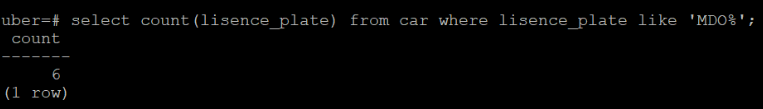
\includegraphics[width=7cm]{Fig 4.3.4.png}
    \caption{String matching query in PSQL}
    \label{fig:4.3.4}
\end{figure}

Above is the result that is supposed to be obtained by the tool. Instead, due to the case mismatching in the wrapper, there are no matches found, and incorrect results are obtained as shown below:
%Insert Fig 4.3.5
\begin{figure}[htp]
    \centering
    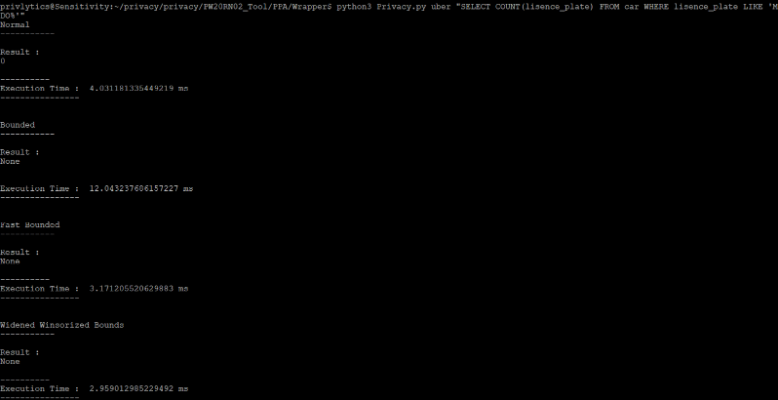
\includegraphics[width=7cm]{Fig 4.3.5.png}
    \caption{Tool error with string matching query}
    \label{fig:4.3.5}
\end{figure}

This error has been debugged in the wrapper by the evaluators, although if unnoticed, could have resulted in complications down the line, hindering the tool’s usage. The snapshot provided displays the output of the corrected wrapper. Since the size of the records to be queried is small (due to the WHERE clause in the query), effective differential privacy cannot be guaranteed by the tool, as shown in the results below, where the Bounded mechanism shows no difference as compared to the normal query execution. The accuracy also varies for each algorithm.
%Insert Fig 4.3.6
\begin{figure}[htp]
    \centering
    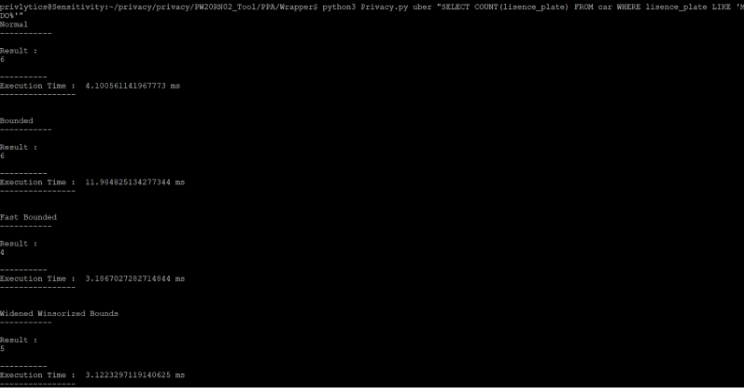
\includegraphics[width=7cm]{Fig 4.3.6.png}
    \caption{Output of string matching query on debugging}
    \label{Fig:4.3.6}
\end{figure}

The wrapper also results in erroneous execution for other queries, especially those which include string matching within multiple nested clauses. It is imperative to note that while the normal and Bounded execution takes place without a glitch, the tool breaks down and fails to execute the FastBounded and Winsorized algorithms. This can be attributed to the selection of bounds by these two algorithms, which select lower and upper bounds based on the outermost attribute of the nested query and hence, may be responsible for violation of PostgreSQL semantics.
%Insert Fig 4.3.7
\begin{figure}[htp]
    \centering
    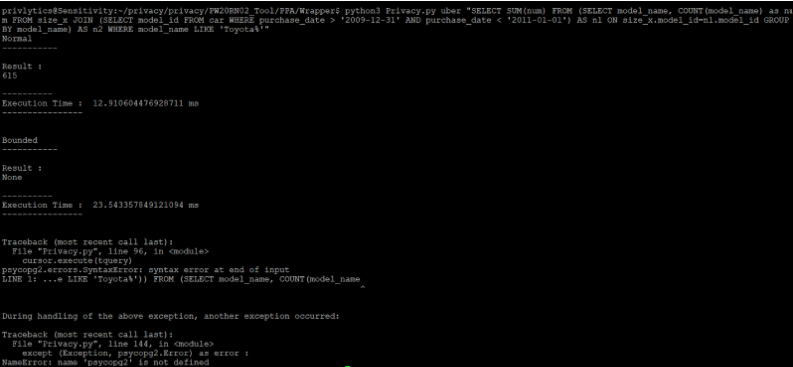
\includegraphics[width=7cm]{Fig 4.3.7.png}
    \caption{Wrapper error - I}
    \label{Fig:4.3.7}
\end{figure}

The wrapper also fails in its handling of queries with the aggregate functions in a nested clause. This is because the wrapper looks for the type of aggregate in the outermost query clause and ignores the subqueries. For example, the query, \texttt{SELECT working\textunderscore hours FROM driver JOIN (SELECT driver\textunderscore id, SUM(price) AS sum\textunderscore p FROM completeride GROUP BY driver\textunderscore id) AS n1 ON driver.driver\textunderscore id=n1.driver\textunderscore id WHERE sum\textunderscore p>500} returns ‘8’ working hours on all the mechanisms without the addition of appropriate noise (as seen in Fig. 13), since the wrapper only checks for an aggregate function in the outermost clause and ignores the nested clauses. The result returned is hence not differentially private and could result in a breach of privacy.
%Insert Fig 4.3.8
\begin{figure}[htp]
    \centering
    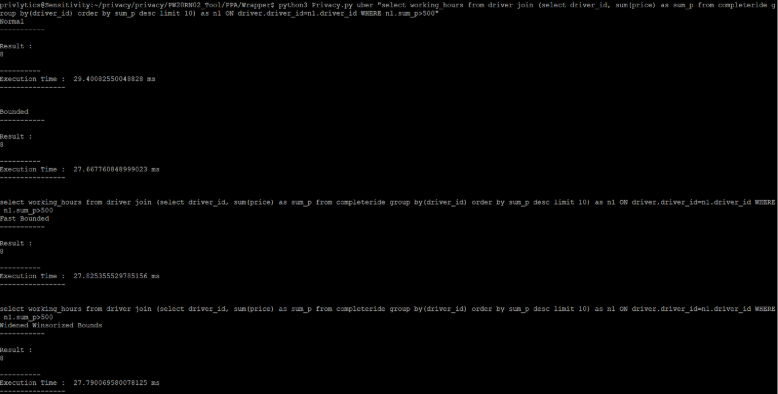
\includegraphics[width=7cm]{Fig 4.3.8.png}
    \caption{Wrapper error - II}
    \label{Fig:4.3.8}
\end{figure}

The tool was also tested with queries containing GROUP BY clauses that brought to light a glaring error. The wrapper fails to work for queries which apply aggregation functions like SUM, AVG, VAR, STDEV in the query clause with the GROUP BY construct. However, this error only arises when the GROUP BY construct is part of the outermost query. This is because of the function in place to set bounds which rewrites the query to fetch MIN and MAX on the attribute queried. It does so using a simple rewriting that does not consider the presence of a GROUP BY clause. For example, the lower bound for a query - \texttt{SELECT AVG(working\textunderscore hours) FROM driver GROUP BY avg\textunderscore ratings}, is defined by the rewriting as \texttt{SELECT MIN(working\textunderscore hours) FROM driver GROUP BY avg\textunderscore ratings}. This returns multiple values due to the presence of grouping resulting in malfunctioning of the wrapper since the function requires a single bound. The query results are displayed below:
%Insert Fig 4.3.9
\begin{figure}[htp]
    \centering
    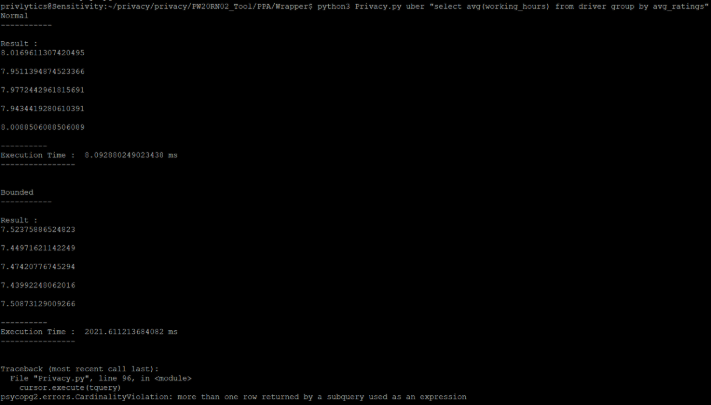
\includegraphics[width=7cm]{Fig 4.3.9.png}
    \caption{Wrapper error - III}
    \label{Fig:4.3.9}
\end{figure}

However, the wrapper functions well with queries that use COUNT as the aggregation function with GROUP BY as seen below :
%Insert Fig 4.3.10
\begin{figure}[htp]
    \centering
    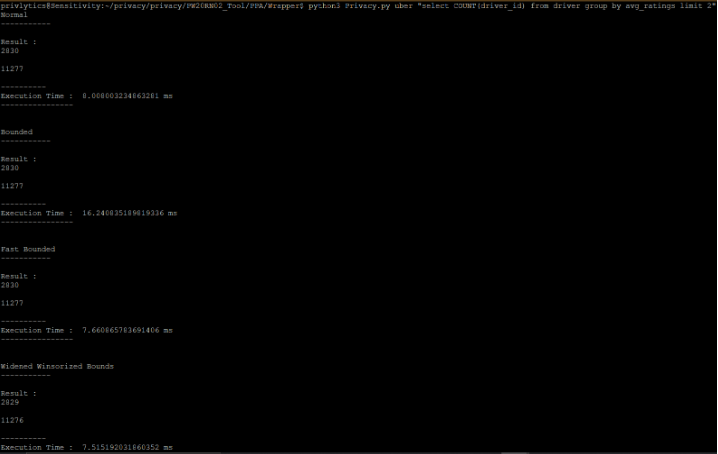
\includegraphics[width=7cm]{Fig 4.3.10.png}
    \caption{GROUP BY query with the COUNT aggregate}
    \label{Fig:4.3.10}
\end{figure}

The last test performed to check functioning was to evaluate if the (modified) tool was indeed preserving privacy under all circumstances. A query that was a blatant violation of privacy was chosen for the same: \texttt{“SELECT SUM(price) FROM completeride WHERE ride\textunderscore id = 5”}, and this query was passed to the tool. It is surprising to note that while the Bounded algorithm returns \texttt{“None”}, indicating that the query indeed violates privacy, the FastBounded and Winsorized mechanisms return random values that vary with every execution of this query. This can be attributed to the selection of bounds by these two mechanisms, due to which the wrapper malfunctions.
%Insert Fig 4.3.11
\begin{figure}[htp]
    \centering
    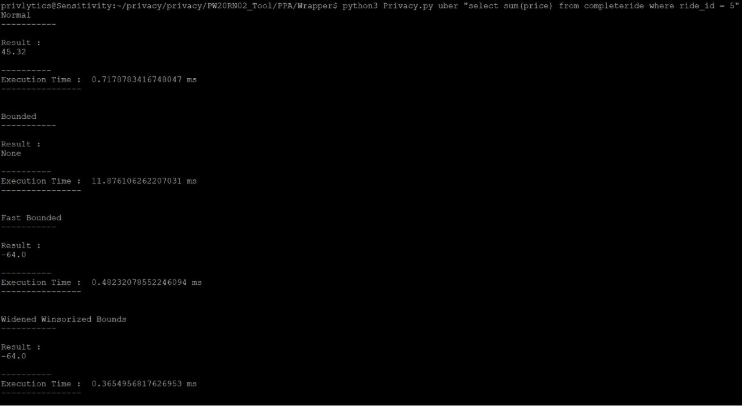
\includegraphics[width=7cm]{Fig 4.3.11.png}
    \caption{Wrapper error - IV}
    \label{Fig:4.3.11}
\end{figure}

It is imperative to state that the wrapper and tool do work efficiently on most of the queries that are generally used in the industry, albeit some exceptions that aren’t handled. Privacy is preserved in almost all cases, except for a few corner cases as highlighted above. We also see that the tool is more effective in preservation of users’ privacy as compared to the wrapper. Further modifications to the wrapper and tool are beyond the scope of this project. The performance and accuracy claims made by the authors of the wrapper are addressed in the following section, with the appropriate statistical and graphical evidence.

\subsection{Performance and Accuracy Metrics}\label{4.4}
One of the main disadvantages of the tool that the authors of the wrapper address is the performance overhead of the tool’s ApproxBounds mechanism, leading to the tool being almost 500 times slower than a normal query. They also claim to have solved this trade-off by introducing a new mechanism - FastBounded, as elaborated upon in the Tool Algorithms section. The authors further claim to have a significant reduction in performance overhead of the tool with their mechanism. This section aims to address these claims and prove or disprove the same with strong statistical and graphical evidence. 
\newline
The precise claims made by the authors are as follows:
\begin{itemize}
    \item A considerable improvement in performance overhead, such that the execution times of the FastBounded queries does not exceed 250x (with x being the execution time of the same query, in a non-differentially private environment)
    \item The accuracy is defined as: x ± 0.2x, or the Margin of Error (MoE) defined at 20\%.
\end{itemize}

Along with testing the performance of the tool and the wrapper, the same metrics were evaluated for the Widened Winsorized mechanism as well, to check if it held up to the same standards or surpassed expectations. The performance and accuracy thresholds remained constant throughout the evaluation process.

In order to test for performance and accuracy metrics, only the queries that provided results without any errors were considered. These were grouped according to whether they were simple, nested or join queries. Each query was passed to the tool 10 times, and the average execution time and result was recorded and used in this evaluation. The queries are similar to the ones executed to check the functioning of the tool (refer previous section) and each type (i.e, simple, nested and join) had at least 10 different queries significant from a real-world perspective.
\newline
\newline
\textbf{Performance Overhead}

The performance was measured by the time taken by each mechanism to execute the same query. This was repeated 10 times each, and the average of the ten execution times obtained was assigned as the resulting time for each mechanism. This was done for Simple, Nested and Join queries. Graphs of these execution times were plotted for each query in each category.

It is surprising to note that none of the algorithms show high performance overhead for nested and join queries, in fact they are comparable with the execution time of the non-differentially private query. This can be attributed to the fact that in most nested clauses, the size of the data points to be analysed significantly reduces and hence do not incur a large performance overhead. Although the reasoning may not apply for certain join conditions, the low performance overhead across mechanisms turns out to be a major advantage of the tool. The graphs for Nested and Join Queries illustrate the same, as shown below.

\begin{figure}[htp]
    \centering
    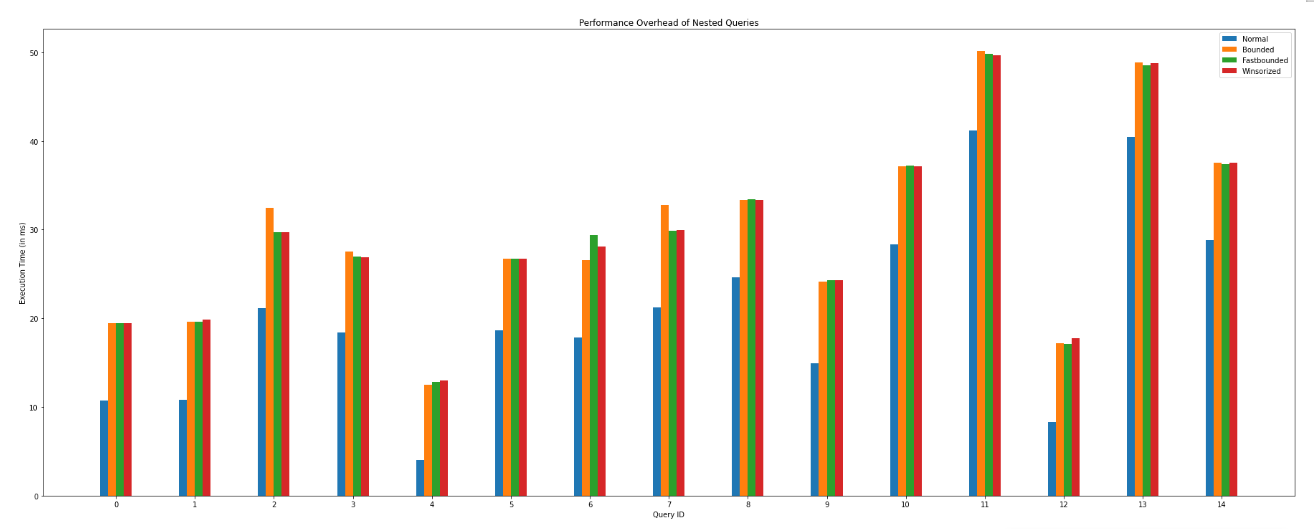
\includegraphics[width=11cm]{Fig 4.4.1.png}
    \caption{Performance overhead for Nested queries}
    \label{Fig:4.4.1}
\end{figure}

\begin{figure}[htp]
    \centering
    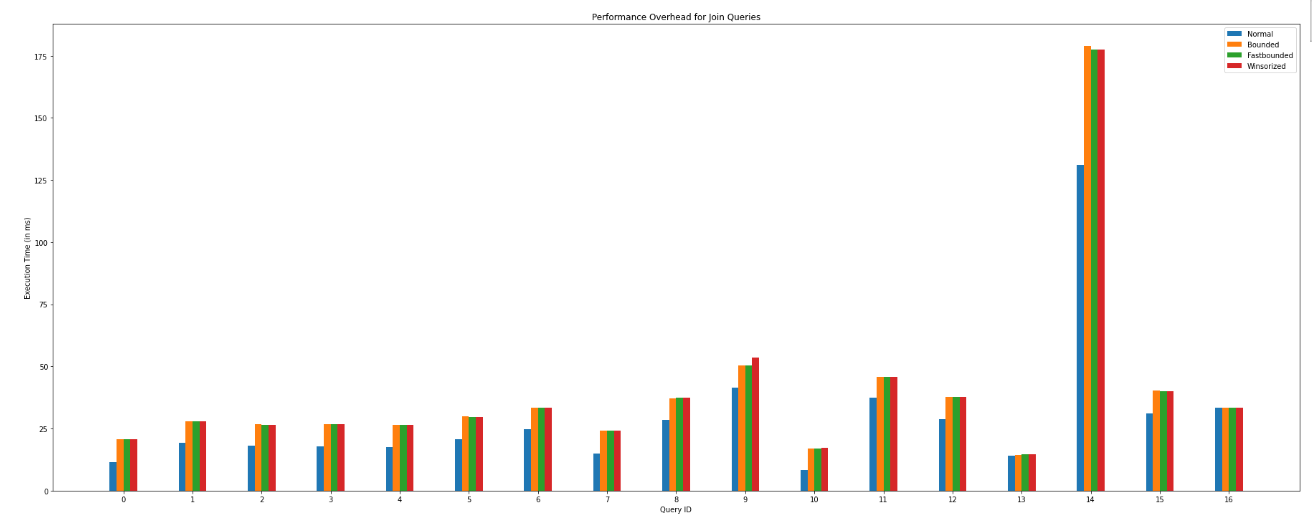
\includegraphics[width=11cm]{Fig 4.4.2.png}
    \caption{Performance overhead for Join queries}
    \label{Fig:4.4.2}
\end{figure}

Regarding the simple queries, the general performance overhead of the Bounded mechanism is extremely high and incomparable with that of the other two mechanisms. With regard to the FastBounded and Winsorized mechanisms, the former does show greater improvement in overhead, however, there isn’t an enormous difference between the two. An example of such a  query is \texttt{SELECT SUM(price) FROM completeride}. The statistical evidence is as follows, with “exec\textunderscore time” representing the average number of milliseconds, and “mode” representing the mechanism used:

\begin{figure}[htp]
    \centering
    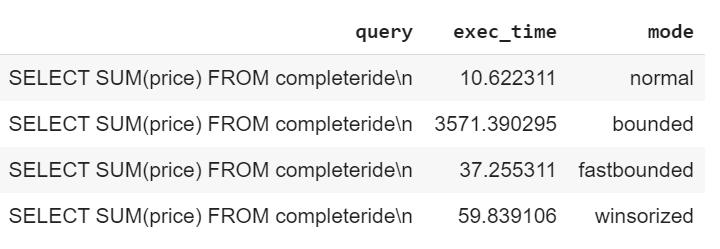
\includegraphics[width=5cm]{Fig 4.4.3.png}
    \caption{Execution times for Simple queries}
    \label{Fig:4.4.3}
\end{figure}

Bounded has an extremely high performance overhead, and takes almost 350 times longer to execute. FastBounded and Winsorized however, are exceptionally faster, lowering the overhead incurred by a factor of almost 60.

A graph was also plotted to see the general performance overhead for each category. This is in accordance with the analysis done for each individual category.

\begin{figure}[htp]
    \centering
    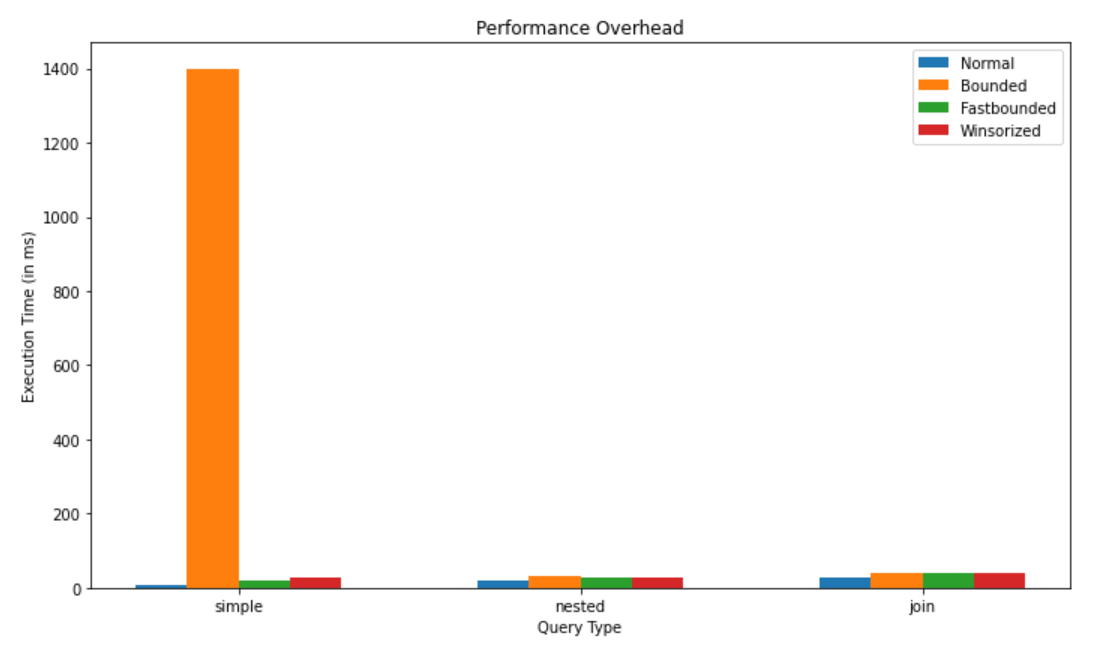
\includegraphics[width=10cm]{Fig 4.4.4.png}
    \caption{Performance overhead per category of queries.}
    \label{Fig:4.4.4}
\end{figure}

From this analysis, it can be conclusively stated that the new mechanisms don’t guarantee a performance overhead for all types of queries, but do provide immense improvement with respect to simple queries.
\newline
\newline
\textbf{Accuracy - Margin of Error}

With regard to the accuracy of the tool and wrapper’s results, the Margin of Error (MoE) was set at 20\% (as per the author’s claim) and used as the metric to measure the accuracy. It is important to note that all queries that violated privacy (i.e, returned a \texttt{‘None’} for the differentially private mechanisms) were not considered while measuring accuracy. The remaining queries were executed 10 times for each mechanism and the average result of which was considered for analysis. Similar to the process followed for evaluation of the tool’s performance, the queries were grouped into the three categories - Simple, Nested and Join, in order to perform analysis.

In nested queries, it was observed that all but one queries had an error rate lesser than 2\% for all mechanisms. Amongst these queries, the Winsorized mechanism shows a slightly higher error (1-1.5\%), which is due to the bounds being selected as the 15th and 85th percentiles. However, there is a glaring exception. The query, \texttt{SELECT COUNT(driver\textunderscore id) FROM completeride WHERE (driver\textunderscore id IN (SELECT driver\textunderscore id FROM driver WHERE (lisence\textunderscore plate IN (SELECT lisence\textunderscore plate FROM car WHERE model\textunderscore ID = '3INOX77MLSV9766838')))) AND price > 40}, shows an incredibly high error at almost 55\% for the FastBounded mechanism, more than double the threshold, and close to 10\% for the Bounded mechanism. Surprisingly, there is little to no error given by the Winsorized mechanism for the same query.

\begin{figure}[htp]
    \centering
    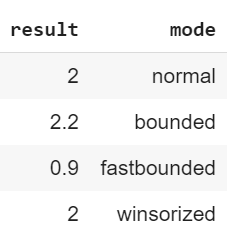
\includegraphics[width=3cm]{Fig 4.4.5.png}
    \caption{Results of Nested query}
    \label{Fig:4.4.5}
\end{figure}

The general consensus of low margins of error is seen across the field, as observed with the queries in the Join category as well. However, there are exceptions as well. The query, \texttt{SELECT COUNT(completeride.driver\textunderscore id) FROM completeride JOIN (SELECT driver\textunderscore id FROM driver JOIN (SELECT lisence\textunderscore plate FROM car WHERE model\textunderscore ID = '3INOX77MLSV9766838') AS n2 ON driver.lisence\textunderscore plate = n2.lisence\textunderscore plate) AS n1 ON completeride.driver\textunderscore id = n1.driver\textunderscore id AND price > 40}, has high error at around 15\% for the Bounded and Winsorized mechanisms, and almost 5\% for the FastBounded mechanism. 

It’s interesting to note that the join query is essentially the same as the nested query highlighted above, but is semantically different. However, the accuracies vary by a large amount, leading to the inference that for queries involving joins, the FastBounded mechanism works faster as compared to the same query written without join clauses.

\begin{figure}[htp]
    \centering
    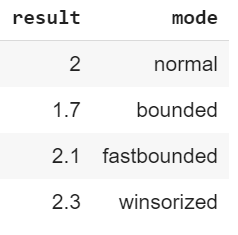
\includegraphics[width=3cm]{Fig 4.4.6.png}
    \caption{Results of Join query - I}
    \label{Fig:4.4.6}
\end{figure}

Another exception to the standard, is \texttt{SELECT COUNT(n1.driver\textunderscore id) FROM (SELECT driver\textunderscore id, working\textunderscore hours FROM driver)AS n1 JOIN (SELECT driver\textunderscore id, SUM(price) FROM completeride GROUP BY driver\textunderscore id) AS n2 ON n1.driver\textunderscore id=n2.driver\textunderscore id AND n1.working\textunderscore hours>8 AND n2.SUM>400}, which crosses the threshold value for the Bounded mechanism, with an MoE of 25\%. The Winsorized mechanism has an error of exactly 20\%, which is also much higher than the FastBound’s 5\% error rate.  The actual results of the same are as follows.

\begin{figure}[htp]
    \centering
    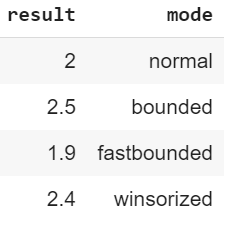
\includegraphics[width=3cm]{Fig 4.4.7.png}
    \caption{Results of Join query - II}
    \label{Fig:4.4.7}
\end{figure}

Simple queries seem to provide the best results, with margins of error for all mechanisms well within the limit. However, the Bounded mechanism shows the highest error rates among all mechanisms, peaking at 14.5\%.

Along with analysis of each category, graphical evidence is also needed in a more general scenario, in order to draw suitable conclusions. This is done using a graph plotted for average error versus the category of queries, grouped by the mechanisms.

\begin{figure}[htp]
    \centering
    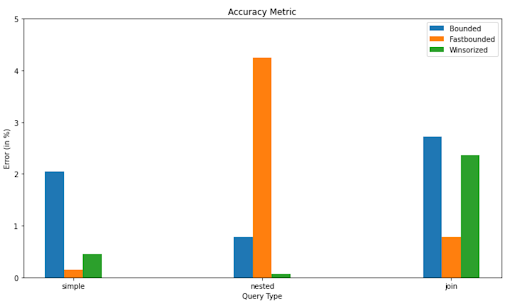
\includegraphics[width=10cm]{Fig 4.4.8.png}
    \caption{Error grouped by category}
    \label{Fig:4.4.8}
\end{figure}

The graph leads to the inference that in general, the tool provides results well within the margin of error, and thus, holds up to the claims made by the authors with regard to accuracy.

\subsection{Usability and General Evaluation}\label{4.5}
This section addresses the general evaluation of the tool, with a bird’s eye view. The usability of the tool involves seeking answers to questions regarding the user-friendliness, ease of understanding and installation, the documentation, and reporting of bugs and errors faced.

Although the installation process is taxing and has to be done multiple times, without a comprehensive README with instructions, once installed, the tool is quite user-friendly. The added bonus of the wrapper allows users with no prior knowledge of the tool’s workings and semantics to also benefit. The execution involves just a single line command, with the name of the database and the normal SQL queries passed as command line arguments to the parser, which enhance the tool’s usability. The tool, without the wrapper, and it’s documentation, is available open source on GitHub, allowing anyone to clone the repository and use it. The documentation is brief, but provides links to relevant material that provide more insight on the tool and the fundamentals behind its working.

The wrapper is adaptable, and anyone with knowledge of its functioning, can make suitable modifications to improve it or debug it, as we did while evaluating. Additionally, the tool can be used on any suitably large database, generalizing its applications to adapt to any industry. All these factors make the tool an important asset to any service provider, allowing them to gain significant insight from data while simultaneously disallowing any sort of breach on an individual’s privacy.

\section{Conclusion}\label{5}
The project has successfully tested the differential privacy tool developed by Google and the modifications made to it by Sriniketh M. Shenoy and Vikram G. on a real-world database and completed a comprehensive evaluation of the claims made by providing statistical and graphical evidence of the same.

The evaluation proves the efficiency of the modifications made to the tool in handling most queries that are industry relevant, while pointing out the shortcomings and improving upon a few of the same. The wrapper fails to handle queries with the aggregate functions nested, queries with grouping clauses and the ones that use string matching. The latter has been fixed with a few modifications to the wrapper by the evaluators.

The evaluation also brings to light that while the wrapper significantly improves the performance overhead, the Bounded mechanism preserves the users’ privacy more effectively. The improvement in performance overhead comes with a compromise on user privacy. A modification using the Widened Winsorized Mechanism has been implemented for the same.

While the build procedure to install the tool is extensive and exhaustive, once built, the tool has an easy to understand, user-friendly interface made possible by the wrapper developed. Although it possibly compromises user privacy in some cases, the tool sufficiently handles most industry relevant queries.

\section{Future Scope}\label{6}
Evaluation of the tool brought to light a few queries that the wrapper is incapable of handling. Extensions to the tool to handle all of these queries would make this approach to achieving differential privacy a more complete solution.

The tool could be made to support complex queries with nested aggregate functions. The solution could lie in query parsing to include sub-queries and employ the ANON functions of the tool on these sub queries as well.

The tool could also be enhanced to handle queries with GROUP BY constructs. The current version only handles GROUP BY in combination with a COUNT aggregate in the outermost query or in a nested clause, as described in the section 4.3.

This project also tried modifying the query processing in the wrapper to support queries with GROUP BYs in combination with any aggregate in simple as well as complex queries. The modification processed the query to set bounds as follows:
\newline
\newline
Consider the query:
\newline
\newline
\texttt{SELECT model\textunderscore name, avg(model\textunderscore year) FROM size\textunderscore x AS s JOIN (SELECT model\textunderscore id FROM car WHERE curr\textunderscore condition=3) AS n1 ON s.model\textunderscore id=n1.model\textunderscore id GROUP BY model\textunderscore name;}
\newline
\newline
The above query is processed to set the lower bound as follows. The upper bound is similarly set with a 0.85percentile cut-off .
\newline
\newline
\texttt{SELECT percentile\textunderscore cont(0.15) within group(order by model\textunderscore year) FROM size\textunderscore x AS s JOIN (SELECT model\textunderscore id FROM car WHERE curr\textunderscore condition=3) as n1 on s.model\textunderscore id=n1.model\textunderscore id}
\newline
\newline
While the tool executes efficiently over such processing for queries with GROUP BY constructs, this method comes with heavy compromise on accuracy. The Margin Of Error far exceeds the allowed 20\% which is why this approach is impractical and unreliable and hence, wasn’t committed. An alternative approach with better merit could be devised for the same.

A new concept to enforce differential privacy could be explored upon to further optimize the performance overhead and compensate the data loss incurred due to bounding. In addition, there is room for significant accuracy improvements through the implementation of Gaussian noise or other mathematical functions and theorems.

\begin{acks}
We would like to express our profound gratitude to our mentor and guide, Dr. Rahul Nagpal, for always providing us with encouragement and wisdom, and without whom this project would not have been successful. We would also like to thank Navraj Singh for being a constant source of support and arranging meetings and presentations without hesitation. This project would not have taken flight without the entire team at the Parallel Systems Research Lab, to whom we are forever indebted. Last but not the least, we would like to thank the Computer Science and Engineering department at PES University, for always inspiring us to conduct frequent research and inculcating a problem-solving discipline in all its students.
\end{acks}

%Unable to figure this out
%Added citation formats for thesis and diff priv paper
%How to cite seniors' report?

%%Johnson, N. M. (2018). Towards Practical Privacy-Preserving Data Analytics. UC Berkeley. ProQuest ID: Johnson\_berkeley\_0028E\_18485. Merritt ID: ark:/13030/m51w0cqm. Retrieved from https://escholarship.org/uc/item/72j4b4n5

\bibliographystyle{ACM-Reference-Format}
\bibliography{bibliography}

\appendix
\section{Sensitivity Formulae}\label{Appendix. A}
Differential privacy provides a formal guarantee of indistinguishability. This guarantee is defined in terms of a privacy budget \begin{math}\epsilon\end{math}—the smaller the budget, the stronger the guarantee. The formal definition of differential privacy is written in terms of the \textit{distance d(x,y)} between two databases, i.e. the number of entries on which they differ: \begin{math}d(x, y) = |i : x_i \neq y_i|\end{math}. Two databases x and y are neighbors if \textit{d(x, y) = 1}. A randomized mechanism \begin{math}\kappa : D^n \rightarrow R preserves (\epsilon; \delta)\end{math}-differential privacy if for any pair of neighboring databases \begin{math}x, y \in D^n\end{math} and set \textit{S} of possible outputs:
\begin{center}
    \begin{math}
        Pr[\kappa(x) \in S] \leq e^\epsilon Pr[\kappa(y) \in S] + \delta
    \end{math}
\end{center}
Differential privacy can be enforced by adding noise to the non-private results of a query. The scale of this noise depends on the sensitivity of the query. The tool considers two different measures of sensitivity; global and local and chooses a third, derived sensitivity - elastic.
\newline

\subsection{Global Sensitivity}
\subsubsection{Definition}
\textit{It is defined as the difference in the results of a query on any two neighbouring databases.}
For \begin{math}f: D^n \rightarrow R^d \end{math}and all \begin{math}x, y \in D^n\end{math}, the global sensitivity of \textit{f} is
\newline
\begin{center}
    \begin{math}
        GS_f = max||f(x) - f(y) || 
    \end{math}
    \hspace{2cm} \textit{where x,y : d(x,y) = 1}
\end{center}
\newline
\newline
\subsubsection{Global Stability}
\textit{A transformation T: }\begin{math} D^n \rightarrow D^n \end{math} \textit{is c-stable if for }\begin{math} x, y \in D^n\end{math} \textit{such that d(x,y) = 1, d(T(x), T(y)) }\begin{math}\leq c\end{math}

\subsection{Local Sensitivity}
\subsubsection{Definition}
\textit{It is defined as the difference in the results of a query on the true database and any of its neighbouring database.}
For \begin{math}f: D^n \rightarrow R^d \end{math}and \begin{math}x \in D^n\end{math}, the local sensitivity of \textit{f at x is}
\newline
\begin{center}
    \begin{math}
        LS_f = max||f(x) - f(y) || 
    \end{math}
    \hspace{2cm} \textit{where y : d(x,y) = 1}
\end{center}

\subsubsection{Local Stability}
\textit{A transformation T: }\begin{math} D^n \rightarrow D^n \end{math} \textit{is locally c-stable for true database x if for }\begin{math} y \in D^n\end{math} \textit{such that d(x,y) = 1, d(T(x), T(y)) }\begin{math}\leq c\end{math}

\subsection{Elastic Sensitivity}
Elastic sensitivity is an upper bound on the local sensitivity and is hence computationally less expensive. Figure \ref{A.3.1} lists the complete definition.
\begin{figure}[htp]
    \centering
    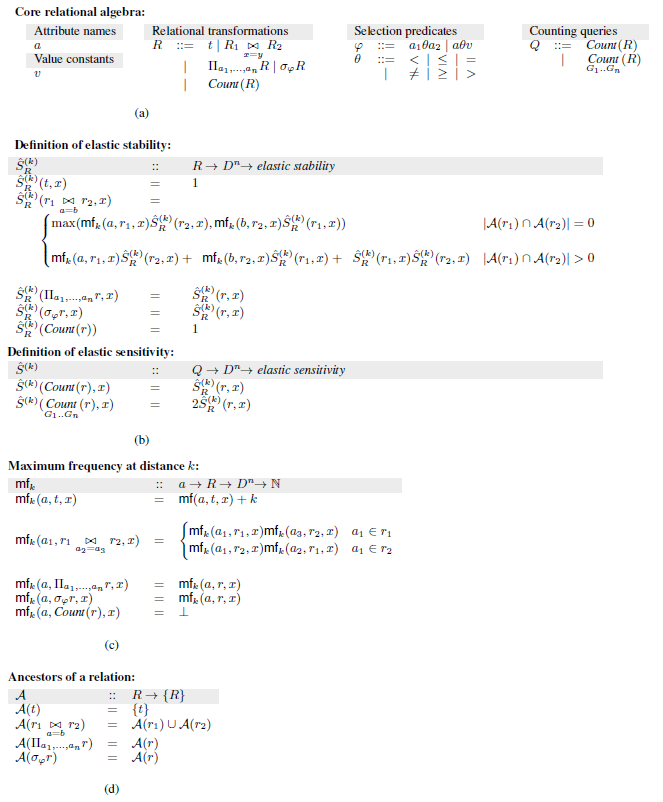
\includegraphics[width=8cm]{ES.PNG}
    \caption{(a) syntax of core relational algebra; (b) definition of elastic stability and elastic sensitivity
at distance k; (c) definition of maximum frequency at distance k; (d) definition of ancestors
of a relation.}
    \label{A.3.1}
\end{figure}
\newline
For a query with elastic sensitivity \textit{S} returning value \textit{v} the Laplace Mechanism releases \begin{math} v + Lap(S/\epsilon) \end{math} where \begin{math}\epsilon\end{math} is the privacy budget allocated to the query. The privacy budget is the threshold after which the tool refuses to return answers.

\section{Sensitivity Bounds for the Google tool}\label{Appendix. B}
The sensitivity of a particular aggregate function is determined by the Google tool, making use of the lower and upper bounds set in order to calculate its value. As mentioned in the above section, the Laplace noise added is scaled to this sensitivity.

Given below are the formulae to calculate sensitivities of each of the aggregate functions the tool supports. 

\begin{figure}[htp]
    \centering
    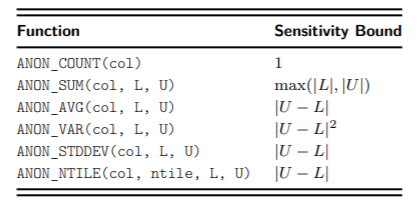
\includegraphics[width=5cm]{appendix1.png}
    \caption{Sensitivities for Aggregate Functions}
    \label{fig:aggregate_sensitivities}
\end{figure}

\section{Threshold Function}\label{Appendix. C}
The ApproxBounds algorithm used by the tool to calculate bounds makes use of histograms to do the same. The data points are placed in bins of appropriate sizes and Laplace noise is added to the count of each bin. To select the lower and upper bounds, the bins with minimum and maximum count, both exceeding a threshold value, is respectively chosen. This threshold function is as follows: 
\begin{equation}
    t = \frac{1}{\epsilon}log(1 - P^{\frac{1}{B-1}})
\end{equation}
The function uses parameters P and B. B refers to the count of histogram bins whereas P is the probability of not selecting a false positive. The ApproxBounds function uses up half of the privacy budget in order to set bounds, while the second half is used for differentially private aggregation.

%\section{List of Figures}
%\listoffigures
\end{document}
\endinput
%%
%% End of file 'ppa.tex'.
